\documentclass[1p, review]{elsarticle}\usepackage[]{graphicx}\usepackage[]{color}
%% maxwidth is the original width if it is less than linewidth
%% otherwise use linewidth (to make sure the graphics do not exceed the margin)
\makeatletter
\def\maxwidth{ %
  \ifdim\Gin@nat@width>\linewidth
    \linewidth
  \else
    \Gin@nat@width
  \fi
}
\makeatother

\definecolor{fgcolor}{rgb}{0.345, 0.345, 0.345}
\newcommand{\hlnum}[1]{\textcolor[rgb]{0.686,0.059,0.569}{#1}}%
\newcommand{\hlstr}[1]{\textcolor[rgb]{0.192,0.494,0.8}{#1}}%
\newcommand{\hlcom}[1]{\textcolor[rgb]{0.678,0.584,0.686}{\textit{#1}}}%
\newcommand{\hlopt}[1]{\textcolor[rgb]{0,0,0}{#1}}%
\newcommand{\hlstd}[1]{\textcolor[rgb]{0.345,0.345,0.345}{#1}}%
\newcommand{\hlkwa}[1]{\textcolor[rgb]{0.161,0.373,0.58}{\textbf{#1}}}%
\newcommand{\hlkwb}[1]{\textcolor[rgb]{0.69,0.353,0.396}{#1}}%
\newcommand{\hlkwc}[1]{\textcolor[rgb]{0.333,0.667,0.333}{#1}}%
\newcommand{\hlkwd}[1]{\textcolor[rgb]{0.737,0.353,0.396}{\textbf{#1}}}%

\usepackage{framed}
\makeatletter
\newenvironment{kframe}{%
 \def\at@end@of@kframe{}%
 \ifinner\ifhmode%
  \def\at@end@of@kframe{\end{minipage}}%
  \begin{minipage}{\columnwidth}%
 \fi\fi%
 \def\FrameCommand##1{\hskip\@totalleftmargin \hskip-\fboxsep
 \colorbox{shadecolor}{##1}\hskip-\fboxsep
     % There is no \\@totalrightmargin, so:
     \hskip-\linewidth \hskip-\@totalleftmargin \hskip\columnwidth}%
 \MakeFramed {\advance\hsize-\width
   \@totalleftmargin\z@ \linewidth\hsize
   \@setminipage}}%
 {\par\unskip\endMakeFramed%
 \at@end@of@kframe}
\makeatother

\definecolor{shadecolor}{rgb}{.97, .97, .97}
\definecolor{messagecolor}{rgb}{0, 0, 0}
\definecolor{warningcolor}{rgb}{1, 0, 1}
\definecolor{errorcolor}{rgb}{1, 0, 0}
\newenvironment{knitrout}{}{} % an empty environment to be redefined in TeX

\usepackage{alltt}
\usepackage{xcolor}      % use if color is used in text


\usepackage{endnotes}
\usepackage{graphicx}   % need for figures
\usepackage{verbatim}   % useful for program listings
\usepackage{hyperref}   % use for hypertext links, including those to external documents and URLs
\usepackage[section]{placeins}
\usepackage{tikz}
\usepackage{fontspec}
\usepackage{fixltx2e}
\usepackage{lineno,hyperref}

\usepackage{pgfplots}
%\pgfplotsset{compat=newest}
%\usepackage{pst-plot,pst-func} 
\usepackage{amsmath}
\usepackage{microtype}

\usetikzlibrary{decorations.text,backgrounds,pgfplots.groupplots,decorations.markings}
\usepgfplotslibrary{fillbetween}

\definecolor{nice_blue}{HTML}{377EB8}
\definecolor{nice_green}{HTML}{4DAF4A}
\definecolor{nice_purple}{HTML}{984EA3}
\definecolor{nice_red}{HTML}{E41A1C}
\definecolor{nice_orange}{HTML}{FF7F00}



%\usepackage[margin=0.5in]{geometry}
\let\footnote=\endnote

%\setromanfont{Frutiger LT Std}


\newcommand{\appropto}{\mathrel{\vcenter{
  \offinterlineskip\halign{\hfil$##$\cr
    \propto\cr\noalign{\kern2pt}\sim\cr\noalign{\kern-2pt}}}}}

\newenvironment{allpgftextsans}{%
  \let\oldpgftext=\pgftext
  \def\pgftext##1{\oldpgftext{\sffamily##1}}
}{}

\pgfplotsset{
    ggplot graphs/.style={
        domain=0:12
        ,xmin=0
        ,xmax=12
        ,ymin=0
        ,ymax=12
        ,axis lines*=left
        ,xtick=\empty
        ,ytick=\empty
        ,every axis y label/.style={
            at={(axis description cs:0.09,.5)}
            ,rotate=90
            ,anchor=south},
        }
        ,every axis x label/.style={
            at={(axis description cs:0.5,0.1)}
            ,anchor=north}
        }
%         cycle list={
%             ultra thick, orange, no markers, smooth\\
%         },
%         shift function/.style 2 args={
%             x filter/.code={\pgfmathparse{\pgfmathresult+##1}},
%             y filter/.code={\pgfmathparse{\pgfmathresult+##2}}
%         },
%         /tikz/tangent line/.style={
%             ultra thick, black, shorten <=-4cm, shorten >=-4cm,
%             insert path={(tangent.west) -- (tangent.east)}
%         },
%         /tikz/indicator lines/.style={
%             thin, densely dashed
%         },
%         /tikz/point/.style={
%             fill,
%             radius=2.5pt,
%         },
%         project point on axes/.code={
%             \pgfplotsset{/pgfplots/after end axis/.code={
%                 \draw [indicator lines]
%                 (tangent-|{rel axis cs:0,0}) 
%                 node [anchor=east] {$x_2^*$} 
%                 -| (tangent|-{rel axis cs:0,0})
%                 node [anchor=north] {$x_1^*$};
%             }}
%         },
        /tikz/label node/.style={
            font=\small,
            align=left,
            anchor=west
        }
    }
}

% \tikzset{
%         tangent point/.style={
%             sloped,
%             name=tangent,
%             pos=#1
%         },
%         tangent point/.default=0.5
% }


\modulolinenumbers[5]

%\journal{Child and Youth Services Review}

%%%%%%%%%%%%%%%%%%%%%%%
%% Elsevier bibliography styles
%%%%%%%%%%%%%%%%%%%%%%%
%% To change the style, put a % in front of the second line of the current style and
%% remove the % from the second line of the style you would like to use.
%%%%%%%%%%%%%%%%%%%%%%%

%% Numbered
%\bibliographystyle{model1-num-names}

%% Numbered without titles
%\bibliographystyle{model1a-num-names}

%% Harvard
%\bibliographystyle{model2-names.bst}\biboptions{authoryear}

%% Vancouver numbered
%\usepackage{numcompress}\bibliographystyle{model3-num-names}

%% Vancouver name/year
%\usepackage{numcompress}\bibliographystyle{model4-names}\biboptions{authoryear}

%% APA style


%% AMA style
%\usepackage{numcompress}\bibliographystyle{model6-num-names}

%% `Elsevier LaTeX' style
%\bibliographystyle{elsarticle-num}
%%%%%%%%%%%%%%%%%%%%%%%

\makeatletter
\def\ps@pprintTitle{%
 \let\@oddhead\@empty
 \let\@evenhead\@empty
 \def\@oddfoot{}%
 \let\@evenfoot\@oddfoot}
\makeatother
\IfFileExists{upquote.sty}{\usepackage{upquote}}{}
\begin{document}

\begin{frontmatter}

  \title{Constrained Parenting Decisions:\\ Toward a General Model of Child Maltreatment\tnoteref{mytitlenote}}

%\title{Elsevier \LaTeX\ template\tnoteref{mytitlenote}}
\tnotetext[mytitlenote]{Prepared for likely submission to the Child and Youth Services Review. Other possibilities (in order of preference) include Child Malreatment, and Social Services Review.}

%% Group authors per affiliation:
%\author{Joseph A. Mienko\fnref{myfootnote}}
  \author{Joseph A. Mienko}
  \address{University of Washington, School of Social Work}
  \ead{mienkoja@uw.edu}
%\address[mysecondaryaddress]{Box 359476, Seattle, Washington 98195-9476}
%\fntext[myfootnote]{Since 1880.}

%% or include affiliations in footnotes:
%\author[mymainaddress,mysecondaryaddress]{Elsevier Inc}
%\ead[url]{www.elsevier.com}

%\author[mysecondaryaddress]{Global Customer Service\corref{mycorrespondingauthor}}
%\cortext[mycorrespondingauthor]{Corresponding author}


%\address[mymainaddress]{1600 John F Kennedy Boulevard, Philadelphia}
%\address[mysecondaryaddress]{360 Park Avenue South, New York}

  \begin{abstract}
  \textbf{Background}: Standard parental investment models from the biological sciences and economics suggest that parents can be expected to care for their children subject to personal characteristics (e.g. altruism) and resource constraints (e.g. money). While previous research has clearly established links between personal characteristics, resources, and maltreatment behaviors, the field lacks any examples of formal attempts to test the predictions of these models with respect to maltreatment behaviors. The goal of this paper is to test a biologically and economically informed model of behaviors associated with child maltreatment. 
  
  \textbf{Methods}: I make use of data from the National Survey of Early Childhood Health (NSECH), the Consumer Expenditure Survey (CES), and the American Time Use Survey (ATUS). Information from these surveys was used to estimate measures of altruism, parental efficiency, income, and other control variables identified in previous NSECH studies. We calculated a dependent measure as the probability that all reported discipline strategies would be Type-II strategies. All of our covariates were subjected to Bayesian Model Averaging (BMA) across quasibinomial GLMs to determine the most probable set of covariates.
  
  \textbf{Results}: The BMA results estimate that the model with the highest posterior probability is a model which only includes the household and parental investments (household altruism) and the natural logarithm of their annual income. In other words, households with higher levels of altruism and higher incomes tend to report higher levels of discipline strategies that are not associated with maltreatment. Our measure of efficiency was rejected from the BMA process and is a weak, insignificant predictor when added to our final model. Results are discussed in terms of implications for social work practice and child welfare practice in particular. 
  
  \end{abstract}

  \begin{keyword}
  Income \sep Child maltreatment \sep Family Characteristics \sep Physical violence
  \end{keyword}

\end{frontmatter}

\begin{knitrout}
\definecolor{shadecolor}{rgb}{0.969, 0.969, 0.969}\color{fgcolor}\begin{kframe}


{\ttfamily\noindent\color{warningcolor}{\#\# Warning: package 'ggplot2' was built under R version 3.1.3}}

{\ttfamily\noindent\color{warningcolor}{\#\# Warning: package 'reshape2' was built under R version 3.1.3}}

{\ttfamily\noindent\color{warningcolor}{\#\# Warning: package 'Hmisc' was built under R version 3.1.3}}

{\ttfamily\noindent\color{warningcolor}{\#\# Warning: package 'RColorBrewer' was built under R version 3.1.3}}

{\ttfamily\noindent\color{warningcolor}{\#\# Warning: package 'extrafont' was built under R version 3.1.3}}\end{kframe}
\end{knitrout}


\linenumbers

\section{Introduction and Theoretical Background}

The purpose of this paper is to formally specify a general theory of child maltreatment. The conclusion of this paper is that child maltreatment is inextricably linked to resource constraints. As such, we tend to see a relationship between a parent’s tendency to maltreat her child and the parent’s relative position in the wealth distribution of a given society. Specifically, a parent on the lower end of a wealth distribution will tend to exhibit an increased probability of maltreating her child relative to parents at the higher end of a wealth distribution. The central thesis of this paper is that maltreatment is the normal consequence of parenting decisions made under household resource constraints. While child maltreatment may be undesirable, in most cases it is not pathological. Recognition of this basic distinction has important implications for child welfare policy and practice. 

The basic relationship between wealth and child maltreatment is well-established in child welfare literature with previous studies establishing links between resource constraints and substantiated allegations of child maltreatment as well as general involvement with the child welfare system \citep{Gil1970, Pelton1981, Pelton1994, Russell1984, Sedlak1996, Stith2009, BergerAndWoldfogel2004}. Studies examining administrative data sets of low-income populations (e.g. TANF recipients) have also shown that exogenous resource-decreasing shocks such as welfare-reform \citep{Courtney2005} or welfare sanctions \citep{Slack2007} will tend to increase a family's probability of child welfare system involvement. Other studies have exploited experimental income support programs to address income endogeneity problems inherent in other studies and still find an inverse relationship between family income and the probability of child maltreatment \citep{Cancian2013, Fein2003}. While there is a paucity of research examining connections between income and child maltreatment outside of the US \citep{Cameron2006}, the evidence from the US seems to suggest a strong and reliable relationship between child welfare system involvement and resource constraints. 

While the literature provides multiple examples of research establishing a link between resources constraints and child maltreatment, the field is lacking in attempts to formally specify a mechanism to explain this relationship. Two exceptions to this rule include \citet{Brandon1999} and \citet{Brandon2001}. In each of these studies, microeconomic models are proposed which outline the manner in which parental resource constraints can lead to maltreatment. The former study suggests that maltreatment is mainly effected by a parent's level of altruism, the latter suggests that maltreatment is a function of how efficiently a parent uses her available resources. Both effects would be subject to income constraints. In this paper, I propose a variation on the models proposed by \citet{Brandon1999} and \citet{Brandon2001} followed by an attempt to test key predictions of the model\footnote{Students of social welfare may initially be taken back by the use of economic models to understand the phenomenon of child maltreatment. Historically, social welfare scholars and other non-economic social scientists have tended to approach theory development as a means of organizing broad constructs or ideas to explain experimental or survey data sources. Economists, on the the other hand, have tended to view theory development as a process analogous to theory development in the physical sciences. As such, in much the same way that an astrophysicist seeks to explain the motion of the planets through mathematical equations, economists have tended to rely on a large body of established mathematical theory in order to explain interactions between humans. While the current paper will not rely heavily on formal mathematical theory, I will show how the conclusions and major concepts of economic theory are still relevant and applicable to the current problem.}. Before describing this model in detail, I will begin by a brief overview of theory from human ethology and neuroscience which serves as first principles for the model proposed in this paper.    

\section{Human Ethology - Why do Humans Engage in Parenting Activities?}

While a full review of the nature vs. nurture debate is beyond the scope of this analysis, this paper proceeds from an assumption that human beings are simultaenously biological \emph{and} social beings \citep[see for example][]{Plomin1994, Ridley2003}. In other words, human beings are not born as a \emph{tabula rasa}. We come pre-wired to engaged in certain activities such as learning languages, consuming nutrients, and engaging in bipedal locomotion. These activities are certainly moderated by the environment in which a human finds himself, but there is no doubt that our genetic makeup helps us to engage in these activities regardless of our environmental circumstances. Basic evolutionary theory shows us that such behaviors exist \emph{because} they helped our genes to evolve to their present state. 

One type of behavior that enabled our genes to survive is parenting behavior and parental altruism in particular. As described in such seminal works as \citet{Hamilton1964} and \citet{Trivers1974}, parental altruism can be defined as those behaviors requiring the investment of time or other resources in a child in a way that benefits the child (in terms of her fitness as a future mate) but comes at a cost to the parent (in terms of her fitness as a future mate). This does not preclude the parent from receiving some sort of benefit from the altruistic act. \citet{Stuebe2010}, for example, find that breastfeeding decreases a mother's long term risk of developing certain chronic diseases. To the extent that an increased survival probability would allow a mother to produce more offspring, she can be viewed as benefiting from the activity to some extent. However, when considering the costs associated with breastfeeding (in terms of caloric loss, the opportunity cost of not bearing other children, etc.), there may be a net cost to the mother's long term fitness. In such situations, parental behavior is said to be altruistic. 

The evolutionary explanation for such behaviors is that by engaging in such altruistic acts to her own children, a parent is increasing the survival probability of her own children and thus increasing the survival probability of her own genes (i.e. those genes that she has passed on to her child). Of course, the parent does not consciously strategize in these behaviors to increase the probability that her genes will survive. Throughout evolution, however, the genes that have survived predispose her to act altruistically. These genes survived \emph{because} they were effective at promoting the survival of her genes. 

Biology does not, however, predispose parents to act altruistically indefinitely. Under periods of extreme scarcity, animals (and humans) will reliably engage in triaging activities in which they will fail to invest in children if it appears likely that investments in that child will come at the expense of another child more likely to survive the scarcity (including future children). This point is well articulated in \citet{Chagnon1983} where Chagnon's fieldwork revealed a Yanomam{\"o} female who killed her newborn child for the sake of her older child who was still nursing. Indeed, \citet{Daly1988} surveyed a database of 60 anthropological ethnographies finding that a majority of the societies engaged in infanticide. Where reasons for the infanticide were provided, almost 90 percent of the reasons were consistent with triaging activities. Until relatively recently in our past, such activities could also be seen in Western societies. \citet{Milner1998} cites an 1860 British newspaper article noting that it had become commonplace for London police to routinely find abandoned infants in the park or other public places. He goes on to cite another British article referring to the large-scale infanticide noting that Middlesex had become a ``carnival of slaughter''. While infanticide is an extreme example, human behavior tends to exist along spectrums and it is reasonable to assume that many parental investment decisions exist along a continuum from optimal to infanticide. As described in more detail below, this threshold will exhibit some heterogenieity across societies. For the purposes of this paper, however, I assume that a threshold exists at some point along this continuum. Beyond this point, parental investment decisions can be considered to be maltreative\footnote{Here, I use the word ``maltreative'', used here as an adjective describing care which is characterized by violence or neglect without regard to malice. Such an adjective is important for the framework presented in this paper as I wish to avoid categorization of behaviors by way of adjectives such as ``abusive'' or ``neglectful'' and I also wish to avoid the inherent presence of malice in the use of an adjective such as ``malicious''. While other candidate adjectives exist (e.g. \emph{laesive} from the Latin adjective \emph{laesus} meaning injured), I have chosen ``maltreative'' due to the relative semantic comfort that most of my readership will find with this word.}.    

\section{Parental Decision-Making - How do Parents Make Decisions About their Children?}

Understanding human behavior, of course, requires a recognition of human agency - the conscious ability of humans to make decisions about how they interact with their world\footnote{To be clear, I am explicitly agnostic about \emph{how} humans make such decisions. Here, I am only stating that humans \emph{do} make such decisions.}. While the field of neuroscience is still new and has only begun to develop a model of parental decision-making \citep[see for example][]{Ho2014}, general neuroscientific models of human decision-making provide some insight into how parents may avoid the maltreative threshold described above. Specifically, a growing body of evidence from brain-imaging studies in neuroscience suggests that humans make decisions with both automaticity (yielding the types of decisions that have allowed our genes to survive for millions of years) and as the result of more thoughtful deliberation (yielding the types of decisions that would cause us to avoid killing our children as the result of post-partum depression). 

\citet{Greene2014} outlines a model of this dual-process human brain in which humans are said to possess an automatic mode (primarily driven by structures such as the ventromedial prefrontal cortex) and a manual mode (primarily driven by structures such as the dorsolateral prefrontal cortex). The experimental evidence for this model is well-covered by Greene and will not repeated here. However, Greene demonstrates how a series of experimental studies show that the dual-process theory of the brain implies a dual-process theory of \emph{morality}. The basis of Greene's theory is what he refers to as the Central Tension Principle in which ``characteristically deontological judgments are preferentially supported by automatic emotional responses, while characteristically consequentialist judgments are preferentially supported by conscious reasoning and allied processes of cognitive control[(i.e. manual mode)]''. In simple terms, moral decisions that require cost-benefit analysis and ``thinking'' (i.e. the types of decisions that would tend to lead to optimal parental investment decisions in spite of resource constraints) require humans to engage in manual mode, deliberative thinking. Other moral decisions are made automatically.

In terms of parenting, this paper assumes that our automatic mode tends to serve humans well most of the time. Human's have evolved to, under normal circumstances, care for their children as described above. This means that most of the time, default parental impulses will tend to avoid a Middlesex-style ``carnival of slaughter''. Placing a parent under resource constraints would require that the parent switch to manual-mode thinking and continue to make optimal investments in their child in spite of the sorts of genetic impulses they might feel. However, recent experimental evidence gives us reason to believe that switching to manual-mode thinking becomes difficult under resource constraints. Specifically, cognitive load (i.e. time pressure or a form of resource constraint) has been been observed to decrease manual mode thinking in experimental subjects \citep{Suter2011, Paxton2012}. Other recent research by \citet{Mani2013} suggests that the types of cognitive load that are induced in experimental settings are also induced by reductions in income. Taken as a whole, these recent findings lead to the conclusion that relatively poor parents who are faced with choices of how to invest in their children will tend to rely on automatic mode decision-making processes relative to wealthier parents. Under \emph{extreme} resource constraints we conclude for the purposes of this paper that this tendency will give way to maltreative behaviors. 

\section{Microeconomic Model}

This manuscript considers two types of individuals ($i$): $p$ and $c$
indicating a parent and child respectively. This is a simplifying
assumption made for the purposes of this paper. The model proposed here,
however, readily extends to multiple children and multiple parents as
well as to children of varying ages and genders. The parent's total
well-being is given as $w_p(x_p)$ where $x_p$ is a composite good
consumed by the parent. The child's well-being is given as $w_c(x_c)$
where $x_c$ is a composite good consumed by the child. For the purposes
of this paper, it is assumed that $x_p$ and $x_c$ are private goods. In
other words, $x_p$ is only consumed by $p$ and $x_c$ is only consumed by
$c$. The overall framework utilized here is, however, general enough to
accommodate both private and public goods through the application of a \citet{Gorman1976} type linear technology function.




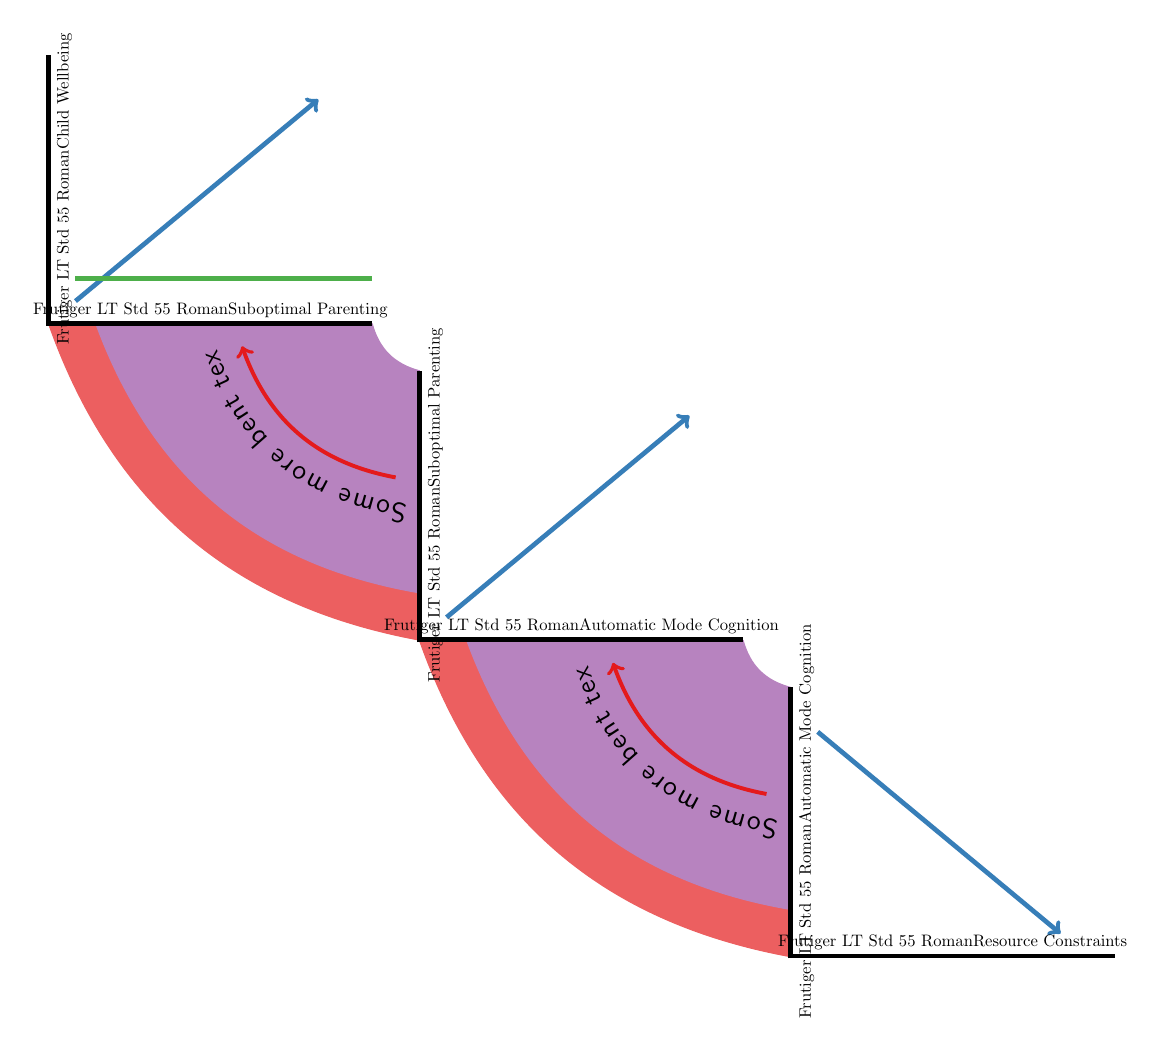
\begin{tikzpicture}[scale=0.6]

\def\myshift#1{\raisebox{2ex}}

\centering
%[axis/.style={very thick, ->, >=stealth'}]
%\def\lam{1}
%\def\k1{0.25}

%\def\b{7}
%\def\m{15}
% \begin{axis}[
%         axis x line=middle
%         ,axis y line=middle
%         ,ymax=0.1
%         ,ylabel=$y$
%         ,xlabel=$x$
%         ,ytick=\empty
%         ,xtick=\empty
%         ]
%     \addplot[domain=0:15, blue, ultra thick, smooth] {(1/\b)*exp(-(((x-\m)/\b)+exp(-((x-\m)/\b))))};



%\tikzstyle{state}=[draw=blue!50, thick, fill=blue!20, minimum size=4mm]
% 
% %abuse
% \node (a1) at (1,0) [state] {}; 
% 
% %sub optimal parenting
% \node (s1) at (2,0) [state] {}; 
% 
% %optimal parenting
% \node (o1) at (5,0) [state] {};
% 
% %abuse
% \node (a2) at (7.85,-6) [state] {}; 
% 
% %sub optimal parenting
% \node (s2) at (7.85,-5) [state] {}; 
% 
% %optimal parenting
% \node (o2) at (7.85,-3) [state] {};

%start of mal optimal parenting
\coordinate (a1o1) at (0,0);
%end of mal optimal parenting
\coordinate (a2o1) at (1,0);
%start of mal manual mode
\coordinate (a1m1) at (7.85,-6.7);
%end of mal manual mode
\coordinate (a2m1) at (7.85,-5.7);
%start of normal optimal parenting
\coordinate (n1o1) at (6.85,0);
%start of normal manual mode
\coordinate (n1m1) at (7.85,-1);




%\draw[name path = abuse_end, bend left]  (a2m) to node [auto] {} (a2o);
%\draw[bend left]  (n1m) to node [auto] {} (n1o);

\filldraw[nice_red!70] (a1m1) to [bend left, auto] (a1o1) -- (a2o1) to [bend right, auto] (a2m1);

\filldraw[nice_purple!70] (a2o1) to [bend right, auto] (a2m1) -- (n1m1) to [bend left, auto] (n1o1);

%start of mal optimal parenting
\coordinate (a1o2) at (0+7.85,0-6.7);
%end of mal optimal parenting
\coordinate (a2o2) at (1+7.85,0-6.7);
%start of mal manual mode
\coordinate (a1m2) at (7.85+7.85,-6.7-6.7);
%end of mal manual mode
\coordinate (a2m2) at (7.85+7.85,-5.7-6.7);
%start of normal optimal parenting
\coordinate (n1o2) at (6.85+7.85,0-6.7);
%start of normal manual mode
\coordinate (n1m2) at (7.85+7.85,-1-6.7);

\node (Na1m1) at (7.85,-3.35) [draw=none,circle,minimum size=6mm,inner sep=0mm] {};
\node (Na1m1_2) at (7.85+3.925,-6.7) [draw=none,circle,minimum size=6mm,inner sep=0mm] {};

\node (Na1m2) at (7.85+7.85,-6.7-3.35) [draw=none,circle,minimum size=6mm,inner sep=0mm] {};
\node (Na1o1) at (3.925,0) [draw=none,circle,minimum size=6mm,inner sep=0mm] {};




\filldraw[nice_red!70] (a1m2) to [bend left, auto] (a1o2) -- (a2o2) to [bend right, auto] (a2m2);

\filldraw[nice_purple!70] (a2o2) to [bend right, auto] (a2m2) -- (n1m2) to [bend left, auto] (n1o2);


\begin{groupplot}[
    group style={
        group size=3 by 3,
        %ylabels at=edge left,
    },
    ggplot graphs,
    ytick=\empty,
    xtick=\empty,
    enlarge x limits=false,
    axis lines*=left,
    %axis x line=left,
    %axis y line=left,
    %every inner x axis line/.append style={|->>}
    axis line style = {line width=2.83464567pt,shorten <=-0.5\pgflinewidth}
]

\nextgroupplot[ymax=6
               ,xmax=6
               ,ylabel=\fontspec{Frutiger LT Std 55 Roman}Child Wellbeing
               ,xlabel=\fontspec{Frutiger LT Std 55 Roman}Suboptimal Parenting]

\addplot[->, nice_blue, line width=2.83464567pt] plot coordinates{
        (0.5,0.5)
        (5,5)};
        
%\begin{axis}
% \addplot[scatter
%         %,color = yellow
%         %,only marks
%         %,mark = triangle*
%         ,mark options={mark size = 4pt
%                         ,rotate=70}
%         ,scatter src=explicit symbolic] coordinates{(5,5)[a]};
%\end{axis}
\addplot[nice_green, line width=2.83464567pt] plot coordinates {
        (0.5,1)
        (6,1)};

\nextgroupplot[hide y axis, hide x axis]
%empty plot spec
\nextgroupplot[hide y axis, hide x axis]
%empty plot spec
\nextgroupplot[hide y axis, hide x axis]
%empty plot spec

\nextgroupplot[ymax=6
              ,xmax=6
              ,ylabel=\fontspec{Frutiger LT Std 55 Roman}Suboptimal Parenting 
              ,xlabel=\fontspec{Frutiger LT Std 55 Roman}Automatic Mode Cognition]
\addplot[->, nice_blue, line width=2.83464567pt] plot coordinates {
        (0.5,0.5)
        (5,5)};

%{(1/\b)*exp(-(((x-\m)/\b)+exp(-((x-\m)/\b))))};
\nextgroupplot[hide y axis, hide x axis]
%empty plot spec
\nextgroupplot[hide y axis, hide x axis]
%empty plot spec
\nextgroupplot[hide y axis, hide x axis]
%empty plot spec
\nextgroupplot[ymax=6
               ,xmax=6
               ,ylabel=\fontspec{Frutiger LT Std 55 Roman}Automatic Mode Cognition
              ,xlabel=\fontspec{Frutiger LT Std 55 Roman}Resource Constraints]
\addplot[->, nice_blue, line width=2.83464567pt] plot coordinates {
        (0.5,5)
        (5,0.5)};
%{((\k1/\lam)*(x/\lam)^(\k1-1))*exp(-((x/\lam)^\k1))};
\end{groupplot}F

% \draw[thick,red] ([shift=(180:1cm)]7.85,0) arc (180:270:1cm);
% \draw[thick,red] ([shift=(180:4.275cm)]7.85,0) arc (180:270:4.275cm);
% \draw[thick,red] ([shift=(180:7cm)]7.85,0) arc (180:270:7cm);
% \draw[thick,red] ([shift=(180:7.85cm)]7.85,0) arc (180:270:7.85cm);
% 
% \draw[thick,red] ([shift=(180:4.275cm)]7.85,0) arc (180:270:4.275cm);
% \draw[thick,red] ([shift=(180:4.275cm)]7.85,0) arc (180:270:4.275cm);
% 
% \draw[thick,red] ([shift=(180:4.275cm)]7.85,0) arc (180:270:4.275cm);
% \draw[thick,red] ([shift=(180:4.275cm)]7.85,0) arc (180:270:4.275cm);


\draw[->
      ,name path = abuse_start
      ,bend left
      ,nice_red
      ,line width=2.83464567*0.5pt
      ,postaction={decorate
                    ,decoration={text along path
                                ,text align=center
                                ,text={|\sffamily\myshift|Some more bent text}}}]  (Na1m1) to node [auto] {} (Na1o1);
      
\draw[->
      ,name path = abuse_start
      ,bend left
      ,nice_red
      ,line width=2.83464567*0.5pt
      ,postaction={decorate,decoration={text along path,text align=center,text={|\sffamily\myshift|Some more bent text}}}]  (Na1m2) to node [auto] {} (Na1m1_2);


\end{tikzpicture}



% \begin{filecontents}{manual_mode.tikz}
% \begin{tikzpicture}
% \def\lam{1}
% \def\k1{0.25}
% \begin{axis}[
%         axis x line=middle
%         ,axis y line=middle
%         ,ymax=1.5
%         ,ylabel=$y$
%         ,xlabel=$x$
%         ,ytick=\empty
%         ,xtick=\empty
%         ]
%     \addplot[domain=0:1.5, blue, ultra thick, smooth] {((\k1/\lam)*(x/\lam)^(\k1-1))*exp(-((x/\lam)^\k1))};
% \end{axis}
% \end{tikzpicture}
% \end{filecontents}
% 
% \begin{filecontents}{optimal_investment.tikz}
% \begin{tikzpicture}
% \def\b{7}
% \def\m{15}
% \begin{axis}[
%         axis x line=middle
%         ,axis y line=middle
%         ,ymax=0.1
%         ,ylabel=$y$
%         ,xlabel=$x$
%         ,ytick=\empty
%         ,xtick=\empty
%         ]
%     \addplot[domain=0:15, blue, ultra thick, smooth] {(1/\b)*exp(-(((x-\m)/\b)+exp(-((x-\m)/\b))))};
% \end{axis}
% \end{tikzpicture}
% \end{filecontents}
% 
% \begin{tikzpicture}
% \node[inner sep=0pt] (manual_mode) at (0,0)
%    {\includegraphics[width=.25\textwidth]{manual_mode.tikz}};
% 
% \node[inner sep=0pt] (optimal_investment) at (5,-6)
%    {\includegraphics[width=.25\textwidth]{optimal_investment.tikz}};
% 
% 
% 
% \end{tikzpicture}






Problems with the definition of child maltreatment have plagued child welfare scholars for decades. While efforts such as the Child Abuse and Treatment Act (CAPTA) (P.L. 92-247) and the uniform definition proposal made by the Centers for Disease Control (CDC) \citep{Leeb2008} have sought to bring consistency to how government officials and researchers think about child maltreatment, no consensus yet exists.

A major contributing factor to the inconsistency in definitions is the legal basis for most of what we think of as child maltreatment. In the flurry of maltreatment legislation that surfaced in the wake of the \citet{Kempe1962} ``discovery'' of the battered child syndrome, the voice of the research community was largely absent in the development of maltreatment legislation. Rather, the discussion was dominated by the medical community which defined the problem imprecisely in terms of social deviance and a defect in the character of parents who engaged in maltreatment \citep{Nelson1986}. Despite the expressed intent of CAPTA to standardize the definition of maltreatment throughout the US, the research and professional community was left with a myriad of statutes which reflected the cultural peculiarities of individual states as opposed to a consensus definition of child maltreatment. In the years that have followed the original passage of CAPTA, US child welfare scholars have been forced to choose between operational definitions of child maltreatment in terms of these variable legal definitions and more traditional psychometric approaches. Although researchers are likely to all utilize the term maltreatment, it is unlikely that researchers are all referring to the same underlying construct \citep{Runyan2005}. 

A common feature of all maltreatment definitions is that they either explicitly or implicitly focus on the actions in which a parent or caretaker has engaged (acts of commission) or in which they have failed to engage (acts of omission). Identifying parental behaviors as maltreative\footnote{Here, I use the word ``maltreative'', used here as an adjective describing care which is characterized by violence or neglect without regard to malice. Such an adjective is important for the framework presented in this paper as I wish to avoid categorization of behaviors by way of adjectives such as ``abusive'' or ``neglectful'' and I also wish to avoid the inherent presence of malice in the use of an adjective such as ``malicious''. While other candidate adjectives exist (e.g. \emph{laesive} from the Latin adjective \emph{laesus} meaning injured), I have chosen ``maltreative'' due to the relative semantic comfort that most of my readership will find with this word.} is certainly a necessary step in describing the phenomenon of child maltreatment, but it is not sufficient. The conceptual diagram displayed in Figure ~\ref{fig:cd} makes this point more clearly. Parental behaviors can be conceptualized as causally emanating from the larger context in which a parent finds themselves. This context includes such factors as the parent's social environment (including their relationship with their child), their genetics, and the laws governing parenting behaviors in a particular society. Parenting behaviors, in turn, can be conceptualized as causally contributing to a child's well-being. Parenting behaviors can increase the child's well-being, but they can also decrease the child's well-being. As a normative rule, parenting behaviors should only be considered maltreative to the extent that they negatively impact the child's well-being. This impact needn't be observed in practice, but it should be observable in principle. A comprehensive definition of child maltreatment should be inclusive of all three of these factors. The purpose of this paper is to propose such a model and test some key predictions of this model. 

The paper is organized as follows: Section \ref{sec:context} outlines some basic assumptions of the model being proposed and justifies the use of a microeconomic model for the child welfare field. Section \ref{sec:theory} presents a non-formal overview of the theoretical framework within the limits of the tolerance which my non-economist readership is likely to have for such an exercise . Section \ref{sec:analysis} describes the my data and overall analytic strategy, and section \ref{sec:results} presents the results of the analysis. Section \ref{sec:discussion} provides a discussion and hypothetical application of the results as well as some concluding remarks.

% \begin{figure}
%   \centering
%   \resizebox {.75\textwidth} {!} {
%     \hbox{\begin{tikzpicture}[->
%                         ,>=stealth'
%                         ,shorten >=1pt
%                         ,auto
%                         ,node distance=5cm
%                         ,ultra thick]
%       \tikzstyle{every state}=[fill=nice_blue
%                                 ,draw=none
%                                 ,text=white
%                                 ,minimum size=2cm
%                                 ,align=center]
%       \node[state] (A)              {Parental \\ Context};
%       \node[state] (B) [right of=A] {Parental \\ Behaviors};
%       \node[state] (C) [right of=B] {Child \\ Wellbeing};
% 
% 
%       \path (A) edge              node {} (B);
%       \path (B) edge              node {} (C);
% 
%     \end{tikzpicture}}
%   }
%   \caption{Conceptual Diagram}\label{fig:cd}
% \end{figure}

\section{Context and Background Assumptions}
\label{sec:context}

\subsection{Why Are Parents? - Remembering Our Biology}
The phrase ``Why Are Parents?'' is an homage to the first chapter of the classic text, ``The Selfish Gene'' by \citet{Dawkins1976} which is titled ``Why Are People?''. Insofar as Dawkins was able to successfully redefine human and animal behavior for a generation of social and physical scientists, I hope that I am not too bold in trying to do the same for child welfare scholars with respect to maltreatment. The economic theory referenced above will serve us well in trying to understand human agency and parenting behavior. However, before we begin that discussion, it is important to spell out some basic assumptions regarding why parents behave as they do in biological terms. 

While the nature vs. nurture debate will probably never present us with a precise numerical answer to the question of what proportion of our human behavior is governed by biology and what is governed by our social environment, there is no doubt that human beings are simultaneously biological \emph{and} social beings \citep[see for example][]{Plomin1994, Ridley2003}. In other words, human beings are not born as a \emph{tabula rasa}. We come pre-wired to engaged in certain activities such as learning languages, consuming nutrients, and engaging in bipedal locomotion. These activities are certainly moderated by the environment in which a human finds herself, but there is no doubt that our genetic makeup helps us to engage in these activities regardless of our environmental circumstances. Basic evolutionary theory shows us that such behaviors exist \emph{because} they helped our genes to survive for millions of years. 

Another type of behavior that enabled our genes to survive is parenting behavior and parental altruism in particular. As described in such seminal works as \citet{Hamilton1964} and \citet{Trivers1974}, parental behaviors are altruistic in that the behaviors require the investment of time and resources in a child in a way that does not directly benefit the parent. These investments do, however, benefit the parent's genes. Each investment that a parent makes in her child increases the probability, however small, that her child will survive to reproduce and allow the continued survival of her genes. Of course, the parent does not consciously strategize in these behaviors to increase the probability that her genes will survive. Throughout the millennia, however, the genes that have survived predispose her to act altruistically. These genes survived \emph{because} they were effective at promoting the survival of her genes. 

Biology does not, however, predispose parents to act altruistically indefinitely. Under periods of extreme scarcity, animals (and humans) will reliably engage in triaging activities in which they will fail to invest in children if it appears likely that investments in that child will come at the expense of another child more likely to survive the scarcity (including future children). This point is well articulated in \citet{Chagnon1983} where Chagnon's fieldwork revealed a Yanomam{\"o} female who killed her newborn child for the sake of her older child who was still nursing. Indeed, \citet{Daly1988} surveyed a database of 60 anthropological ethnographies finding that a majority of the societies engaged in infanticide. Where reasons for the infanticide were provided, almost 90 percent of the reasons were consistent with triaging activities. Until relatively recently in our past, such activities could also be seen in Western societies. \citet{Milner1998} cites an 1860 British newspaper article noting that it had become commonplace for London police to routinely find abandoned infants in the park or other public places. He goes on to cite another British article referring to the large-scale infanticide noting that Middlesex had become a ``carnival of slaughter''. 

\subsection{Dual Process Theory of Morality - Protecting Ourselves from the Carnival}
What mechanism stops us from engaging in a ``carnival of slaughter''? At least part of the answer would appear to come to us from the burgeoning field of experimental philosophy (so-called ``XPhi''). A growing body of evidence from brain-imaging studies in this field suggests that humans make decisions with both automaticity (yielding the types of decisions that have allowed our genes to survive for millions of years) and as the result of more thoughtful deliberation (yielding the types of decisions that would cause us to avoid killing our children as the result of post-partum depression). 

\citet{Greene2014} outlines a model of this dual-process human brain in which humans are said to possess an automatic mode (primarily driven by structures such as the ventromedial prefrontal cortex) and a manual mode (primarily driven by structures such as the dorsolateral prefrontal cortex). The experimental evidence for this model is well-covered by Greene and will not repeated here. However, Greene demonstrates how a series of experimental studies show that the dual-process theory of the brain implies a dual-process theory of \emph{morality}. The basis of Greene's theory is what he refers to as the Central Tension Principle in which ``characteristically deontological judgments are preferentially supported by automatic emotional responses, while characteristically consequentialist judgments are preferentially supported by conscious reasoning and allied processes of cognitive control[(i.e. manual mode)]''. In simple terms, moral decisions that require cost-benefit analysis and ``thinking'' (i.e. the types of decisions that would tend to maximize well-being) require humans to engage in manual mode, deliberative thinking. Other moral decisions are made automatically.

In terms of parenting, our automatic mode tends to serve us well most of the time. Human's have evolved to, under normal circumstances, care for their children as described above. This means that most of the time, default parental impulses will tend to avoid a Middlesex-style ``carnival of slaughter''. One might hope that when parents are placed under resource constraints that they would switch to manual-mode thinking and continue to care for their children in spite of the sorts of genetic impulses they might feel. However, there is additional experimental evidence from the \citet{Greene2014} line of research which suggests that cognitive load (i.e. time pressure or a form of resource constraint) actually leads to a decrease in manual mode thinking \citep{Suter2011, Paxton2012}. Other recent research by \citet{Mani2013} suggests that the types of cognitive load that are induced in experimental settings are also induced by reductions in income. In terms of parenting, it is reasonable for us to conclude from this line of reasoning that poor parents who are faced with choices of how to invest in their children will tend to rely on automatic mode decision-making processes relative to wealthier parents. 

\subsection{The Welfare State - Protecting Citizens from the Carnival}

Since the 19th century, Western society has evolved into a series of social welfare states which also seek to prevent the existence of ``carnival[s] of slaughter''. With respect to the family, governments have come to acknowledge an implicit agreement between parents and children which consists of a fiduciary relationship between parents and children in which children are viewed as principals and parents are viewed as ``...agent[s] of the child's well-being'' \citep[p. 57,][]{TestaAndPoertner2010}. Under this definition, if a parent acts in her own self-interest at the expense of her children's well-being, a principal-agent problem can be said to exist. Moreover, because this principal-agent problem tends to lead to children who are less well-developed and less capable of full participation in society as adults \citep[e.g.][]{BarroEtAl1986}, the problem also produces a negative externality. 

For the purposes of this paper, instances in which this contract is broken down are viewed to be instances of child maltreatment. When children are maltreated, the state is viewed to have a fiduciary obligation to both the child and to the rest of society. The state's obligation to the child is to ensure that actions are being taken to promote the child's well-being. If the parent is unable to fulfill this role, the state is required to act \emph{in loco parentis} or \emph{in place of the parent} to ensure that proper investments are made in the child's human capital. In ensuring that these investments are made, the state also works to maximize social welfare for society as a whole by ensuring that externalities caused by a parent's failure to properly invest in his children are minimized. 

By defining the parent-child relationship in terms of an agreement it should become clearer why a microeconomic theory is particularly appropriate model for household decision-making. Although most of economic theory tends to focus on monetary transactions, this is not the limit of economic theory. For economists, most human decisions and behaviors can be modeled through economic theory. In many cases, the economic or monetary aspect of a given theory is simply used to better explain how individuals engage in any social exchange. As will be shown in more detail below, money is simply a means through which these exchanges are carried out in most human societies - it is a symbolic representation of an agreement.

\subsection{Existing Evidence for the Relationship between Maltreatment and Resource Constraints}
\label{sec:lit}

Previous research has clearly established links between resource constraints and substantiated allegations of child maltreatment as well as general involvement with the child welfare system \citep{Gil1970, Pelton1981, Pelton1994, Russell1984, Sedlak1996, Stith2009, BergerAndWoldfogel2004}. Studies examining administrative data sets of low-income populations (e.g. TANF recipients) have also shown that exogenous resource-decreasing shocks such as welfare-reform \citep{Courtney2005} or welfare sanctions \citep{Slack2007} will tend to increase a family's probability of child welfare system involvement. Other studies have exploited experimental income support programs to address income endogeneity problems inherent in other studies and still find an inverse relationship between family income and the probability of child maltreatment \citep{Cancian2013, Fein2003}. While there is a paucity of research examining connections between income and child maltreatment outside of the US \citep{Cameron2006}. The evidence from the US seems to suggest a strong and reliable relationship between child welfare system involvement and resource constraints. 

Additional support for the theoretical context described above can be seen in descriptive statistics of maltreated children. The theory reviewed in previous sections suggests that the vast majority of human parenting activity is focused on caring for children as opposed to harming them. It is possible then, that many of the parents who are involved with the child welfare system have been trying to effectively parent their children and have failed to do so. A review of evidence concerning serious injuries in Western child welfare systems suggests that this may be the case. For example, the results from the most recent National Incidence Study demonstrate that the majority of maltreatment in the US does not result in serious injury\footnote{While the studies cited here vary in what they consider to be ``serious'' maltreatment, the definitions are similar and generally indicate an instance of maltreatment in which medical attention was required.} \citep{Sedlak2010}. This finding is consistent across prior NIS studies and earlier surveys of child maltreatment in the US \citep[e.g.][]{Gil1970}. Within the Canadian child welfare system, \citet{TrocmeEtAl2007} finds that just 3\% of the substantiated maltreatment reports were severe enough to warrant any medical intervention\footnote{There are, of course, differences between the Canadian and US child protection systems. However, there are inherent cultural similarities between the two countries as well as a common lineage in Elizabethan Poor Law and progressive era children's societies. Furthermore, the overall incidence of child maltreatment in Canada is similar to that of the US. For instance, the 2008 incidence of child maltreatment in the US was 10.3 per 1,000 children in the population \citep{HHS2013} compared with a rate of 14.19 in Canada \citep{TrocmeEtAl2010}. While a difference of 4.6 incidents of maltreatment per 1,000 children is not inconsequential, we can reasonably expect the proportion of serious incidents of child maltreatment in the US to be similar to that of Canada.}. Setting aside problems with reporting and erroneous substantiation practices, one of two possibilities exist for less severe cases: 1) that parents in these cases intend to harm their children and fail to do so (and are thus reported to the child protection authorities), or 2) that parents in these cases try to effectively parent their children and fail to do so (and are thus reported to child protection authorities for some other reason (e.g. inappropriate discipline, failure to provide proper clothing, etc.)). The theory reviewed above is suggestive of the latter.

\section{Proposed Theoretical Model}
\label{sec:theory}

At this point, we have established a genetic predisposition for humans to care for their children, subject to resource constraints. Ethological theories of parental behavior such as those referenced above provide us a means through which we can describe unconscious and involuntary behavior throughout the animal kingdom. \emph{Human} parenting behavior, however, is also purposeful and goal directed. With respect to children, human parents make decisions about how they desire to invest in their children and enact these decisions on their children (or the environment in which their children reside). While some portion of this behavior may stem from unconscious and involuntary genetic impulses, parents also possess human agency which they can use to determine how to best satisfy these impulses - including harmful impulses that they may feel under resource constraints\footnote{To be clear, I am explicitly agnostic about \emph{how} humans make such decisions. Here, I am only stating that humans \emph{do} make such decisions.}. Using the language of \citet{Greene2014}, we can say that humans will use both automatic-mode thinking \emph{and} manual-mode thinking to care for their children. Under extreme resource constraints, however, automatic-mode thinking will tend to yield harmful parental impulses. These resource constraints simultaneously limit the parent's ability to engage in manual-mode thinking which could allow them to see beyond these harmful impulses. At times, resource constraints can become so great that the state must intervene to ensure the well-being of the child.   

While the literature provides multiple examples of research establishing a link between resources constraints (defined as household income) and child maltreatment, the field is lacking in attempts to formally specify models based on this relationship. Two exceptions to this rule include \citet{Brandon1999} and \citet{Brandon2001}. In each of these studies, microeconomic models are proposed which outline the manner in which parental resource constraints can lead to maltreatment. The former study suggests that maltreatment is mainly effected by a parent's level of altruism, the latter suggests that maltreatment is a function of how efficiently a parent uses her available resources. Both effects would be subject to income constraints. In this section, I propose a variation on the models proposed by \citet{Brandon1999} and \citet{Brandon2001} followed by an attempt to test key predictions of the model\footnote{Students of social welfare may initially be taken back by the use of economic models to understand the phenomenon of child maltreatment. Historically, social welfare scholars and other non-economic social scientists have tended to approach theory development as a means of organizing broad constructs or ideas to explain experimental or survey data sources. Economists, on the the other hand, have tended to view theory development as a process analogous to theory development in the physical sciences. As such, in much the same way that an astrophysicist seeks to explain the motion of the planets through mathematical equations, economists have tended to rely on a large body of established mathematical theory in order to explain interactions between humans. While the current paper will not rely heavily on formal mathematical theory, we will show how the conclusions and major concepts of economic theory are still relevant and applicable to the current problem.}. 

\section{Non-Formal Theoretical Specification}

In this paper I consider two types of individuals ($i$): $p$ and $c$ indicating a parent and child respectively. This is a simplifying assumption made for the purposes of this paper. The model proposed here, however, readily extends to multiple children and multiple parents as well as to children of varying ages and genders. The parent's total well-being is given as $w_p(x_p)$ where $x_p$ is a composite good consumed by the parent. The child's well-being is given as $w_c(x_c)$ where $x_c$ is a composite good consumed by the child. For the purposes of this paper, we assume that $x_p$ and $x_c$ are private goods. In other words, $x_p$ is only consumed by $p$ and $x_c$ is only consumed by $c$. The overall framework utilized here is, however, general enough to accommodate both private and public goods through the application of a \citet{Gorman1976} type linear technology function. 

In using the term well-being, I am drawing an implicit equivalence between the term and the traditional concept of utility utilized in standard microeconomic theory\footnote{In economic terms, I assume that well-being (as measured by characteristics which are observable in practice or in principle) is a positive monotonic transformation of an underlying latent utility concept $u_i$, that a person's well-being for two choices $j$ and $k$ is ordinally comparable such that $w_{ij} > w_{ik} \rightarrow u_{ij} > u_{ik}$, and that it is cardinally comparable with $w_{ij} - w_{ik} \rightarrow u_{ij} - u_{ik}$.}. In this way, I am following the line of literature started by \citet{Easterlin1974} which acknowledges that the choices that people make are subject to the context in which an individual finds themselves and that an individual's well-being is derived from more than just increased consumption. This view implies that income-based measures of well-being should be thought of as necessary but not sufficient to the study of well-being \citep{Graham2008}. In general, this paper proceeds from an assumption that well-being can be conceptualized by what philosophers and positive psychologists would refer to as eudaimonia - a higher level of happiness \citep{Kashdan2008} which can be viewed as inclusive of cognitive or hedonic forms of happiness. While this paper does not seek to explicitly test a eudaimonic formulation of well-being in economic models, the reader should be clear that the models and theoretical assumptions presented here are, in the general case, consistent with notions of well-being and happiness that are more familiar to non-economists and social welfare scholars \citep[e.g.][]{Ryff1989} and that these conceptions of well-being do not necessarily reduce to hedonism or require strictly ``rational'' preferences.  

Like the economic conception of utility, well-being can be understood as the level of satisfaction that an individual experiences as the result of consumption and other choices about how to live their lives\footnote{It is important to note that human well-being is not just a function of the items that an individual might purchase or consume; it is more generally a function of an individual's preferences and the choices that individuals make throughout their lives. Talking in terms of composite goods is simply a convenient way of discussing human choices and the constraints (e.g. budgets, etc.) that people have on there choices.}. For my purposes, I consider two composite goods that could be consumed by a child: household-produced investments $x_{ch}$ (e.g. making meals, reading to the child, playing with the child, etc.) and market purchased investments for the child $x_{cm}$ (e.g. childcare, etc.). In this paper, I implicitly follow \citet{Brandon2001} and assume that $x_c = x_{ch} + x_{cm}$ such that $w_c=w(x_{ch},x_{cm})$.

For illustrative purposes\footnote{These figures are for illustrative purposes only. Unless specifically notes, we assume no functional form of the well-being functions proposed in this paper.}, the contours of $w_c$ are shown in Figure ~\ref{fig:plot1}. As in utility theory, the contours are referred to as indifference curves; a two-dimensional representation of our three-dimensional well-being function. A key feature of this graph is the notion of substitution. That is, as the child consumes more of one form of investment, she necessarily consumes less of the other. Movement along any one indifference curve represents a household's trade-offs of one good for another while maintaining a constant level of well-being. As the household investment in a child moves from one curve to the next (i.e. from $w1$, to $w2$, to $w3$), the child's well-being is said to be increasing. The goods that comprise $x_p$ can be assumed to behave in a similar manner. 



\begin{figure}
\centering
%\resizebox{\columnwidth}{!}{
\begin{tikzpicture}

\node at (.75,4.5) {\fontspec{Frutiger LT Std 55 Roman}w\textsubscript{1}};
\node at (1.25,5) {\fontspec{Frutiger LT Std 55 Roman}w\textsubscript{2}};
\node at (1.75,5.45) {\fontspec{Frutiger LT Std 55 Roman}w\textsubscript{3}};
\node[color=nice_green] at (5.35,3.5) {\fontspec{Frutiger LT Std 55 Roman}Well-being};
\begin{axis}[
    %ggplot graphs,
    axis lines*=left,
    ytick=\empty,
    xtick=\empty,
    xmin=0, 
    xmax=12,
    ymin=0, 
    ymax=12,
    %x label style={at={(axis description cs:0.5,-0.1)},anchor=north},
    %y label style={at={(axis description cs:-0.1,.5)},rotate=90,anchor=south},
    xlabel=\fontspec{Frutiger LT Std 55 Roman}Household Produced Investments x\textsubscript{ch}, 
    ylabel=\fontspec{Frutiger LT Std 55 Roman}Market Purchased Investments x\textsubscript{cm},
    axis line style = {line width=2.83464567*0.5pt,shorten <=-0.5\pgflinewidth},
    enlarge x limits=false
]
\addplot [nice_blue, line width=2.83464567pt, smooth] table {wb1.dat};
\addplot [nice_blue, line width=2.83464567pt, smooth] table {wb2.dat};
\addplot [nice_blue, line width=2.83464567pt, smooth] table {wb3.dat};
\addplot[->, nice_green, line width=2.83464567pt] plot coordinates{(7,7)(8.5,9)};
\end{axis}
\end{tikzpicture}
%}
\end{figure}



% \begin{figure}
% <<Figure1, echo=FALSE, cache=TRUE>>=
% 
% #Basic Utility
% x <- c(1, 3, 9)
% y <- c(9, 3, 1)
% 
% wb1 <- data.frame(bezier(x, y, evaluation = 500))
% wb2 <- data.frame(bezier(x+1, y+1, evaluation = 500))
% wb3 <- data.frame(bezier(x+2, y+2, evaluation = 500))
% # 
% # textAnnotations <- data.frame(label = c(paste(expression("w[3]")), "w2", "w3"),
% #                               x = c(1.1, 2.1, 3.1),  # DF of line labels
% #                               y = c(9.4, 10.4, 11.4))
% 
% p1 <- qplot(x = 0:12, y = 0:12, geom = "blank")  # Draw an empty plot
% p1 <- p1 + geom_path(data = wb1, aes(x = x, y = y),  # Add utility 1
%                        size = 1, colour = cols[2])
% p1 <- p1 + geom_path(data = wb2, aes(x = x, y = y),  # Add utility 2
%                        size = 1, colour = cols[2])
% p1 <- p1 + geom_path(data = wb3, aes(x = x, y = y),  # Add utility 3
%                        size = 1, colour = cols[2])
% p1 <- p1 + annotate("segment"
%                     ,x = 7
%                     ,xend = 9
%                     ,y = 7
%                     ,yend = 9
%                     ,colour = cols[3]
%                     ,size = 1
%                     ,arrow = arrow(length = unit(4,"point")
%                                     ,type="closed")
%                     )
% p1 <- p1 + annotate("text",
%                     size=4.23333333228,
%                   
%                     x = 10, y = 7, 
%                       label = "Well-Being", colour = gray(1/2),
%                     family = "Frutiger LT Std 45 Light") #Arrow Label
% 
% 
% p1 <- p1 + annotate("text"
%                     ,size=4.23333333228
%                     ,x = c(1.1, 2.1, 3.1) # DF of line labels
%                     ,y = c(9.4, 10.4, 11.4)
%                     ,label = c(paste(expression(w[1])),
%                                paste(expression(w[2])),
%                                paste(expression(w[3])))
%                     ,parse=TRUE
%                     ,family = "Frutiger LT Std 45 Light")
% # p1 <- p1 + geom_text(data = textAnnotations,  # Add curve labels
% #                        aes(x = x, y = y, label = label, family = "Frutiger LT Std 45 Light"))
% p1 <- p1 + scale_x_continuous(expression(paste("Household Produced Investments ",x[ch])))
% p1 <- p1 + scale_y_continuous(expression(paste("Market Purchased Investments   ",x[cm])))
% p1 <- p1 + theme_classic(base_size = 12, base_family = "Frutiger LT Std 45 Light")
% p1 <- p1 + coord_equal()  # Force fixed x-y relationship
% p1 <- p1 + theme(axis.ticks = element_blank(), #remove numbering
%                    axis.text.y = element_blank(),
%                    axis.text.x = element_blank(),
%                    axis.line = element_line(size = 1)) 
% p1
% @
\caption{Child's Well-Being Function}\label{fig:plot1}
\end{figure}


For this paper I rely on a collective model of the household as first conceptualized by \citet{Chiappori1988}. In a collective model, household members are assumed to cooperate in order to achieve a Pareto efficient distribution of household resources. In this way I break from \citet{Brandon1999} and \citet{Brandon2001} in which a unitary model, in line with \citet{Becker1981}, is assumed to underlie the household decision-making process. While a full review of unitary and collective models of household decision-making is outside of the scope of this paper (see \citet{Chiappori2011} for such a review), unitary models have fallen out of favor in recent years. In general, unitary models suffer from the assumption of a single decision-maker in a given household. In developing a theory of child maltreatment, I propose that a collective approach in which the preferences of the parent (or parents) \emph{and} the preferences of the child (or children) are considered to be analytically preferable to a unitary model in which child preferences are typically ignored. Furthermore, with respect to maltreatment, the basic conclusions of \citet{Brandon1999} and \citet{Brandon2001} still hold under this model. 

I specifically assume that the each member of the household seeks to maximize the household welfare $W$ through a two-stage program. In the first stage of the program, the household identifies a sharing rule $\phi_i$ in which the parent's share of income is governed by a sharing function $\phi_p=\phi(p_p, p_c, y, Z)$ and the child's share of income is governed by a sharing function $\phi_c=y-\phi(p_p, p_c, y, Z)$ where $p_p$ and $p_c$ represent labor-based wages of the parent and child respectively, $y$ represents household income, and $Z$ represents a vector of distribution factors which do not impact parental or child preferences but do influence the manner in which resources are distributed within the household. Such factors could include local child protection laws, the age of the child, cultural factors, and other considerations. The second stage of the program involves each member maximizing a household welfare function $W^i$ according to the following program:  

\begin{align}\label{eqn:stage2}
\begin{split}
\text{max } W^i[w_p(x_p), w_c(x_c)]\\
\text{s.t. } x_i = \phi_i
\end{split}
\end{align}

While some readers may question the implicit human agency afforded to children in the above specification, we find that this approach is preferred to ignoring the preferences of children in the allocation of household resources \citep[as in, e.g.][]{Blundell2007}. As shown by \citet{Sodian2004}, even infants can be shown to exhibit human agency. This point will be well-taken by any reader who has ever parented a newborn child overnight; the preferences of the child as manifest through a desire to feed, play, or engage in other activities at any hour of the day or night clearly impact which household resources are available for the parent and which are available for the child. 

What should be clear from the above discussion is that $p_c=0 \rightarrow \phi_c=x_c/y$. In other words, when $p_c=0$, $\phi_c$ is simply the proportion of household resources expended on the child in stage 1. Some additional resources (some portion of $\phi_p$) may be expended on the child in stage 2 of the program according to a caring parameter $\alpha_p$ (i.e. altruism under \citet{Becker1981}). Under an assumption that $W$ takes a Cobb-Douglas form where $\alpha_p$ is defined as the output elasticity of $w_c$, it can be shown through Roy's identity \citep{Roy1947} that $\alpha$ is simply the proportion of $\phi_p$ which is expended on $x_c$. Thus, for our purposes, we assume that the total household expenditures on $x_c$ are equal to $\alpha_p + \phi_c$. 

\subsection{Graphical Analysis - Connecting Parental Decision Making to Abuse}

Following \citet{Brandon2001} and \citet{Brandon1999}, we assume that a given society sets a minimum well-being threshold $\bar{w}$. When parents invest in their children above this level, society is generally accepting of the parent. When parents invest below this level, the state must intervene to ensure a minimum well-being for the child. Figure ~\ref{fig:plot2} illustrates this point in terms of a well-being production possibility frontier. Each frontier ($F1$ and $F2$) represent the possible ``efficient'' outcomes of parental ($w_p$) and child ($w_c$) well-being that could be produced within two sets of resources. A given household will invest more or less in the child depending on parental preferences $(\alpha_p)$ and the household sharing rule $(\phi_c)$. 

Several points are immediately clear from this diagram. To begin, it can be seen that inefficient production as represented by production bellow $F1$ or $F2$ is not necessarily maltreative production. This is the case of point $A$ which represents a hypothetical household which is inefficiently producing $w_c$ and $w_p$. However, the household is still producing $w_c$ above societal expectations, $\bar{w}$. Sometimes, however, inefficient production does fall below $\bar{w}$. Household $B$ represents such a household. By moving to point $B'$, household $B$ could be brought above $\bar{w}$ within the existing resources of the household. In other words, they could stop maltreating their child without any financial assistance. Such movement might take place, for example, as the result of a drug treatment program in which a substance-abusing parent achieves sobriety and is able to spend more time with their child. Point $C$ represents a point where the parent is efficiently using all of her available resources by investing on $F1$ but is still investing below $\bar{w}$. In such an instance, the state could provide a wealth transfer to the parent and, holding household $(\phi_c)$ and parental preferences $(\alpha_p)$ constant, increase the investment in the child above $\bar{w}$ (to point $C'$). The state could also seek to move the parent from $C$ to $B'$ by trying to change household and/or parental preferences. An example of this might be the application of a parenting intervention to teach the parent new discipline strategies. 

\begin{figure}
\begin{knitrout}\small
\definecolor{shadecolor}{rgb}{0.969, 0.969, 0.969}\color{fgcolor}

{\centering 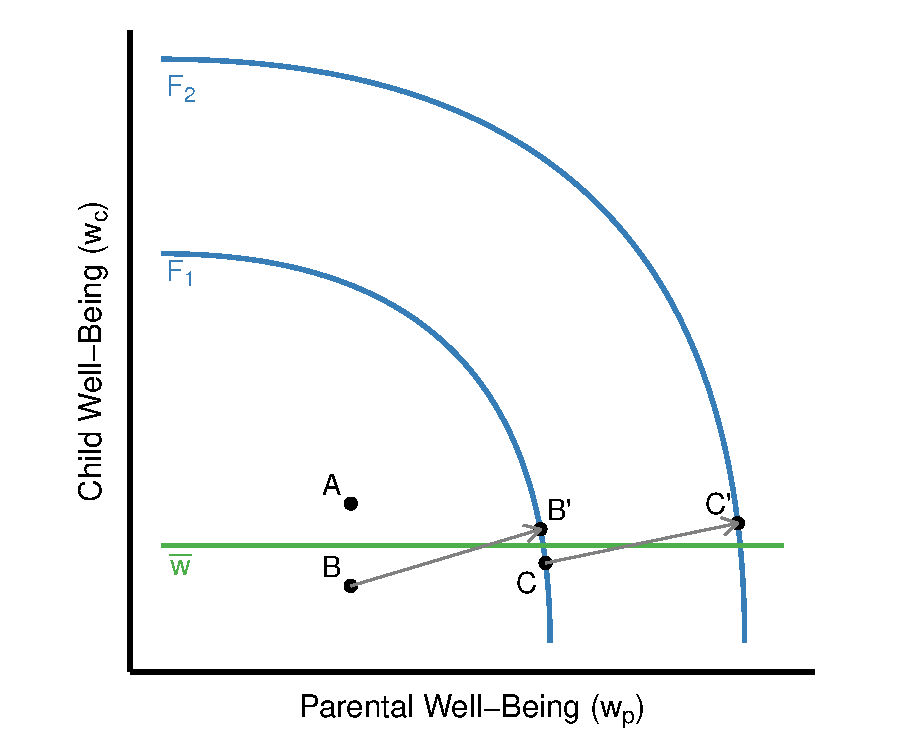
\includegraphics[width=\maxwidth]{figure/Figure2-1} 

}



\end{knitrout}
\caption{Well-Being Production Possibilities}\label{fig:plot2}
\end{figure}

Recall from above, however, that $x_c=x_{ch}+x_{cm}$. Parents not only choose how much to invest in $x_c$, \citet{Brandon2001} argues that the manner in which the parent invests in $x_c$ also matters. Specifically, Brandon argues that maltreatment can be defined as a function of a parent's comparative advantage in child care (i.e. the efficiency $\theta$ with which she spends time, $x_{ch}$, caring for the child) vs. childcare goods and services (e.g. education, nanny service, etc., $x_{cm}$) with some parents having a natural affinity for child care and some parents having a natural affinity for market skills. The basic logic is articulated in Figure ~\ref{fig:plot3} where $\bar{w}$ represents the boundary of minimal accepted investment in a child. The right side of the curve represents the various combinations of time and goods that the state would find it acceptable to have invested in a given child. Here, I also add to the \citet{Brandon2001} model and show how investment options are not infinite for parents. That is, the state will not allow a parent to invest entirely in concrete goods at the expense of providing direct care of the child. The state expects that parents will provide some minimum level of $x_{ch}$ and $x_{cm}$. This is represented by the points at which the investment threshold levels off in the northwest and southeast quadrants of the figure. 

\begin{figure}
\begin{knitrout}\small
\definecolor{shadecolor}{rgb}{0.969, 0.969, 0.969}\color{fgcolor}\begin{kframe}


{\ttfamily\noindent\bfseries\color{errorcolor}{Error: Use 'theme' instead. (Defunct; last used in version 0.9.1)}}\end{kframe}

{\centering 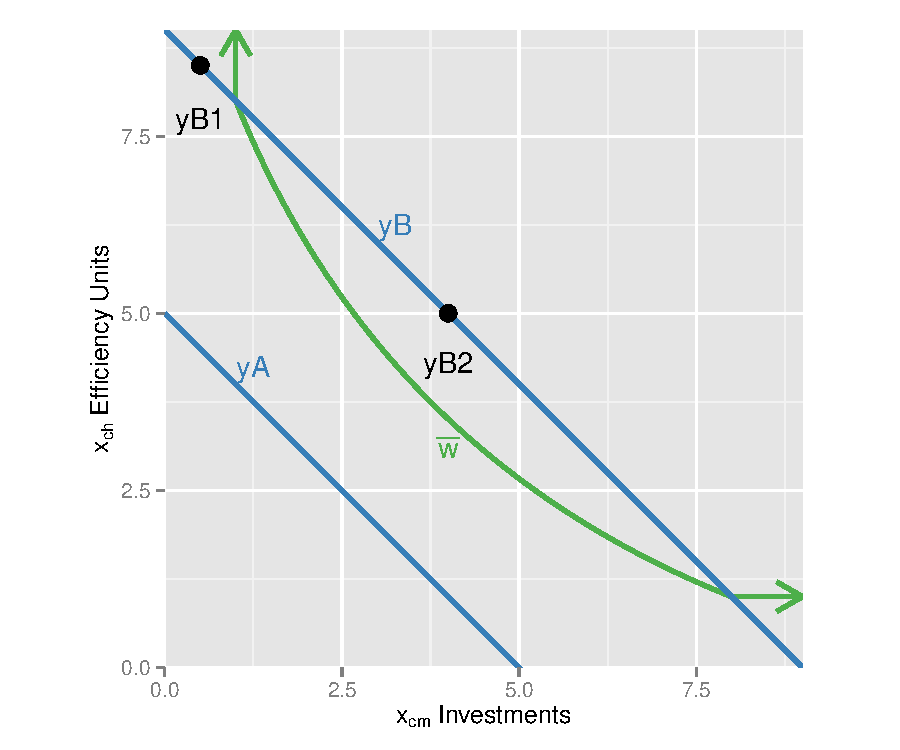
\includegraphics[width=\maxwidth]{figure/Figure4-1} 

}



\end{knitrout}
\caption{Comparative Advantage of Investments}\label{fig:plot3}
\end{figure}

The implication of this chart is that there are some parents who are in the unfortunate position of always falling below this threshold regardless of how efficiently they use their resources. An example would be a parent investing in her child at any point along income line $yA$. Income line $yB$, however, has a slightly different situation. A parent investing in her child at point $yB1$ could (perhaps with the proper educative services) be shown how to invest at a point closer to point $yB2$ which would bring her child into the zone of societal acceptance (the right side of $\bar{w}$). The only way that a parent with income $yA$ can invest in her child in the zone of societal acceptance is to increase her income. 

\subsection{Major Predictions of the Model}

There are many predictions which stem from the model of child maltreatment described above. For our purposes, the major prediction of this model is that the probability $P$ of child maltreatment can be expressed as 

\begin{align}\label{eqn:prediction}
P(w_c < \bar{w})=g(\alpha_p, \phi_c, y, F(\phi_c + \alpha_p, x_c))
\end{align} 

where $F$ is the Farrell output efficiency for a household \citep{Farrell1957} in terms of the inputs $(\phi_c + \alpha_p)$ and output $x_c$. Our model specifically predicts that $P(w_c < \bar{w})$ monotonically decreases as a function of $g$. 

\section{Data and Analytic Strategy}
\label{sec:analysis}

\subsection{Identifying Data}

I am unaware of any single set of data which would allow me to test the maltreatment predictions implicit in Equation ~\ref{eqn:prediction}. In order to test the predictions of this model, we would require access to information concerning the financial resources of given household, the investments they make in their children (in terms of time and market expenditures), and the maltreative behaviors that they employ with their children. As we are seeking to describe \emph{deviations from normal parenting behavior} it is critical that we make use of a nationally representative data set in testing our predictions. Thus, while data sets such as the National Survey of Child and Adolescent Well-Being (NSCAW) provides nationally representative data, such data are limited to children and families who have been referred to child welfare agencies under suspicions of child abuse or neglect and are thus of limited utility here. 

One set of data which meets most of our needs is the National Survey of Early Childhood Health (NSECH). This survey involved telephone interviews with over 2,000 parents with children under 3 years of age in early 2000 (n=2,068). In addition to various demographic factors, the NSECH also collected information on the income of parents and their employment status, the time that children spend in the care of other individuals, the source of the care (childcare provider, etc.), the time that parents spend caring for their children in various activities (story-reading, etc.), and parental discipline strategies, (spanking, time-out, etc.). 

Two barriers exist with the NSECH data: 1) the survey provides information on income, childcare, time-investments, and discipline strategies in ordinal scales which limits our ability to perform basic mathematical operations requisite for our analysis (e.g. summing time investments), and 2) the survey does not indicate whether or not a particular discipline strategy has been assessed as maltreative; only whether or not the parent engages in a particular strategy. The following two sections provide a general overview of how I accommodated these problems. Further details of each component of these (and subsequent steps in my analysis) are available in my GitHub repository \href{https://github.com/mienkoja/qualpaper}{https://github.com/mienkoja/qualpaper} and will also be included as technical appendices when this manuscript is submitted for publication. 

\subsubsection{Combing Data Sets}

The first short-coming is addressed by making use of other nationally representative data sets. Specifically, Bureau of Labor Statistics (BLS) data from the 2003 American Time Use Survey (ATUS) and the 2004 Consumer Expenditure Survey (CE) is utilized. Using this data to develop ``prior'' distributions for each measure, I implement a smoothing algorithm which allows me to treat the data from these surveys as continuous. The algorithm I employ is as follows:

\begin{enumerate}
  \item Match the relevant variables from the NSECH and the relevant BLS survey,  
  \item Visually examine the distribution of the BLS data, 
  \item Calculate the MLE of a reasonable prior for the relevant variable,  
  \item Simulate a sampling distribution of relevant variable with a Monte Carlo function, and 
  \item Sample from the simulated data sets within intervals as identified in the ordinal NSECH data.  
\end{enumerate}

Two exceptions are made to this algorithm. The first exception is in my estimate of the total household expenditures on child care. For this measurement, I utilize CES-based estimates of the average expenditures for childcare in various childcare settings and multiply this by the total hours that NSECH respondents reported that their child spend in the corresponding settings. The variance in the hours reported in NSECH provides us with a continuous measurement of this expenditure without the need to incorporate the variance of a CES-based ``prior''. Also, in estimating a continuous measurement of income, I utilize a distribution as reported in a working paper by \citet{Bandourian2002} which provides me with a reasonable prior distribution for US income. 

\subsubsection{Assumptions Regarding Discipline Strategies}

The second short-coming is addressed in two steps. First, I recall a well-known distinction in discipline strategies which classifies discipline according to the provision of a stimulus (e.g. spanking, yelling, etc.) as compared with the taking of a stimulus (e.g. time-out, removing a toy, etc.). The behaviorist literature classifies these strategies as Type I ($D_I$)and Type II ($D_{II}$) discipline respectively\footnote{These strategies can be analogously classified as positive and negative punishment. This distinction is also similar to authoritarian and authoritative parenting strategies.}. Second, I recall that $D_I$ strategies are generally less-likely to promote child well-being than $D_{II}$ discipline strategies. We know, for instance, that $D_I$ strategies tend to be problematic for parent-child relationships and can sometimes lead to behavioral problems for children including delinquency and aggression \citep{Gershoff2002, Taylor2010}. I thus proceed from an assumption that $D_I$ and $D_{II}$ discipline strategies exist on a continuum of discipline strategies and that $D_I$ behaviors are the sorts of behaviors that are less likely to increase a child's well-being and more likely to create a situation in which $w_c < \bar{w}$. This assumption is bolstered by a line of literature which links $D_I$ parenting strategies to resource constraints \citep{Berger2007, Berger2008, Berger2009, Paxson2002} in a manner similar to the identified link between resource constraints and child maltreatment in the literature reviewed above. Put simply, I assume that as indications of $D_{II}$ behaviors increase, a child will be less likely to be considered maltreated in a given society. 

\subsection{Description of Key Variables}







The variables listed in Equation ~\ref{eqn:prediction} are defined as follows:

\subsubsection{Household Income $(y)$}

Income in the public-use NSECH data is reported in terms of total household income on an 8-point Likert scale starting at $\le 7,500$ and proceeding in increments of 10,000 to $\ge 75,000$. Continuous income is calculated to the algorithm specified above. As income is reported as ``total household income'', depending on the use, I divide the estimated continuous value by the number of adults in the household in order to arrive at an estimate of individual wages for parents who report some employment.    

\subsubsection{Household Resources Devoted to Child Well-Being $(\alpha_p + \phi_c)$}

I do not observe $\alpha_p$ and $\phi_c$ directly in the NSECH data. However, under the assumptions described above, we are able to see that the sum of these parameters is equal to the total household resources devoted to the child $A$ (this can be thought of imprecisely as a measure of ``household altruism'' toward the child). In order to calculate $A$ I take the following steps: 

\begin{enumerate}
  \item Taking the estimate of $y$ calculated above, the count of adults in the home $n_a$, and the estimated number of work hours $t_w$, I estimate the parent's wage $p_p$ as $(y/n_a)/(365.25(t_w))$. For non-working mothers, we value their time at the estimated market rate for child-care calculated from the CES above.   
  \item I then calculate $A$ by summing the total time value that a parent spends on home-based child care $p_px_{ch}$ and the time value of market child care $p_px_{cm}$ and then divide by the time value of the total number of hours in the year $(p_p(365.25)(24))$ such that $A=(p_px_{ch}+p_px_{cm})/(p_p(365.25)(24))$.
\end{enumerate}

\subsubsection{Output Efficiency ($F$)}

I do not observe $F$ directly and there is no way to empirically calculate this value within our available data. I can, however, estimate a distance function using an MLE of the production possibility frontier for $x_{ch}$ and $x_{cm}$. While a detailed discussion of this estimation is beyond the scope of this paper, \citet{Bogetoft2010} provide a thorough overview of the approach. In essence, I make some assumptions about our measure of efficiency $F$ and use this (in conjunction with our estimate of the frontier) to estimate a distance $D$ from the frontier for each household in our data. In this paper, I make use of the \texttt{Benchmarking} package by \citet{Bogetoft2013} which is available in the statistical programming language, R.

\subsubsection{$P(\text{All } D_{II})$}

Since I do not directly observe indications of societally identified maltreatment, I rely on information concerning the discipline strategies of the parent. We specifically calculate for each person, the probability that \emph{all} of their reported discipline strategies would be $D_{II}$. In using this measurement as our dependent measure, we are implicitly assuming that $P(w_c \ge \bar{w}) \appropto  P(\text{All } $D_{II}$)$. 

Parents in the NSECH were asked 5 questions regarding their discipline strategies. The specific question pattern is as follows:

\begin{quotation}
The next questions are about discipline. Parents vary a lot in how they discipline and children also vary in their response to being disciplined. I am going to read a list of methods of discipline parents might use with children (CHILD)'s age. For each, please tell me if you use that method often, sometimes, rarely, or never with (CHILD). First, how about raising your voice or yelling? How about spanking? How about taking away a toy or treat? How about giving a time-out, that is making (CHILD) take a break from whatever activity {he/she} is involved in? How about explaining to (CHILD) why {his/her} behavior is not appropriate.'' 
\end{quotation}

Using this information, I calculated $P(\text{All } D_{II})$ as follows: 

\begin{enumerate}
  \item In order from first to last, I classify the first, second, and last questions as Type I strategies $D_I$ as they are are providing a stimulus to the child. The third and fourth questions are classified as Type II strategies $D_{II}$ as they remove a stimulus from the child. 
  \item I then dichotomize each response for each question. Questions in which a subject answered ``Never'' were coded as 0 and 1 otherwise. 
  \item We then calculate our probability for each subject $k$ as \\ 
  $P_k(\text{All }D_{II_k})=\sum{D_{II_k}}/(\sum{D_{II_k}}+\sum{D_{I_k}})$.
\end{enumerate}

\subsubsection{Additional Variables}

In addition to our key variables of interest, we also consider the use of variables utilized in previous NSECH research concerning discipline strategies. Specifically, \citet{Regalado2004} makes use of child age, maternal race, maternal age, maternal marital status, maternal education, maternal frustration levels, child health, and developmental concerns as potential risk factors in their multivariate analysis. Our current analysis also makes use of the count of children in the household as an additional variable. A descriptive summary of all the identified variables is provided in Table~ \ref{tabdesc}. 


% latex table generated in R 3.1.2 by xtable 1.7-1 package
% Sun Oct 18 16:06:35 2015
\begin{table}[ht]
\centering
\scalebox{1}{
\begin{tabular}{crrrr}
  \hline
 & min & max & $\bar{X}$ & $\tilde{X}$ \\ 
  \hline
$P(\text{All }D_{II})$ & 0.00 & 1.00 & 0.47 & 0.50 \\ 
  $A$ & 0.02 & 1.00 & 0.28 & 0.25 \\ 
  $F$ & 0.40 & 0.94 & 0.82 & 0.84 \\ 
  $y$ & 132.11 & 186747.69 & 36412.74 & 26111.33 \\ 
  Child Count & 1.00 & 4.00 & 2.18 & 2.00 \\ 
  Child Age (mos) & 19.00 & 35.00 & 26.62 & 27.00 \\ 
  White Mother & 0.00 & 1.00 & 0.54 & 1.00 \\ 
  Maternal Age & 17.00 & 49.00 & 29.26 & 29.00 \\ 
  Married Mother & 0.00 & 1.00 & 0.63 & 1.00 \\ 
  Maternal College & 0.00 & 1.00 & 0.48 & 0.00 \\ 
  Maternal Frustration & 0.00 & 1.00 & 0.54 & 1.00 \\ 
  Child Healthy & 0.00 & 1.00 & 0.81 & 1.00 \\ 
  Devolpmental Concerns & 0.00 & 1.00 & 0.79 & 1.00 \\ 
   \hline
\end{tabular}
}
\caption{Descriptive Statistics} 
\label{tabdesc}
\end{table}


\subsection{Statistical Analysis}
All of our covariates were subjected to Bayesian Model Averaging (BMA) across generalized linear models (GLMs) to determine the most probable set of covariates. The details of BMA are beyond the scope of this paper. The reader is directed to \citet{Hoeting1999} for a discussion of the overall approach. Briefly, BMA is a process through which a researcher identifies a set of potential $k$ covariates and a candidate statistical model (e.g. a quasibinomial generalized linear model (GLM)). The analyst then estimates the statistical model for every possible combination of models ($2^k$ models). Each model receives a weighting based on the posterior probability of the model beginning with a prior probability which represents the researcher's beliefs prior to conducting the analysis. For the current problem, I begin with a relatively conservative uniform prior. I utilize a quasibinomial GLM to account for overdispersion in $P(\text{All }D_{II})$. The BMA is implemented via the \texttt{BMA} package authored by \citet{Raftery2009}. 

\section{Results}
\label{sec:results}

The results of the BMA indicate that the ``most probable'' of the $2^k$ fitted models is a model which only includes $A$ and $\log{y}$. Specifically, this model has a posterior probability of 0.472 and the next most-probable model has a posterior probability of 0.16. The estimates for the chosen model are displayed in Table ~ \ref{tabmod}. As can be seen, the probability of choosing all $D_{II}$ strategies is positively and significantly associated with $A$ and $\log{y}$. The results are displayed graphically in Figures ~ \ref{modModelResultGph1} and \ref{modModelResultGph2}. 

% latex table generated in R 3.1.2 by xtable 1.7-1 package
% Sun Oct 18 16:06:35 2015
\begin{table}[ht]
\centering
\scalebox{1}{
\begin{tabular}{rrrrr}
  \hline
 & Estimate & Std. Error & t value & Pr($>$$|$t$|$) \\ 
  \hline
Intercept & -0.9869 & 0.2156 & -4.58 & 0.0000 \\ 
  A & 0.4488 & 0.1115 & 4.02 & 0.0001 \\ 
  y & 0.0807 & 0.0201 & 4.02 & 0.0001 \\ 
   \hline
\end{tabular}
}
\caption{Model Results} 
\label{tabmod}
\end{table}


\begin{knitrout}\small
\definecolor{shadecolor}{rgb}{0.969, 0.969, 0.969}\color{fgcolor}\begin{figure}

{\centering 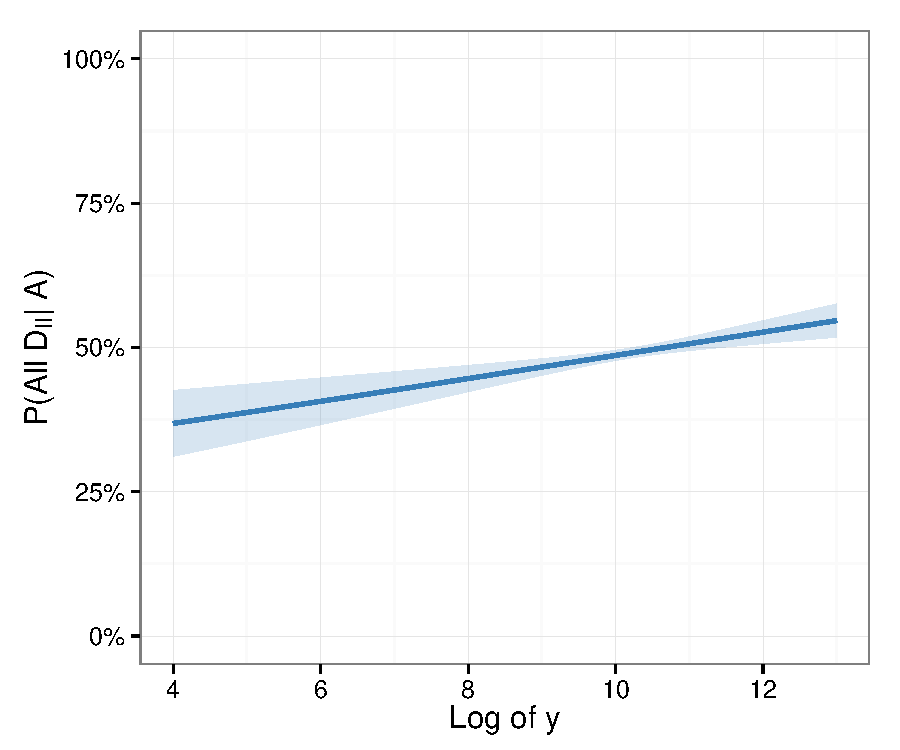
\includegraphics[width=\maxwidth]{figure/ModelResultGph1-1} 

}

\caption[]{$P(\text{All } D_{II})$ as a function of $\log{y}$}\label{modModelResultGph1}
\end{figure}


\end{knitrout}

\begin{knitrout}\small
\definecolor{shadecolor}{rgb}{0.969, 0.969, 0.969}\color{fgcolor}\begin{figure}

{\centering 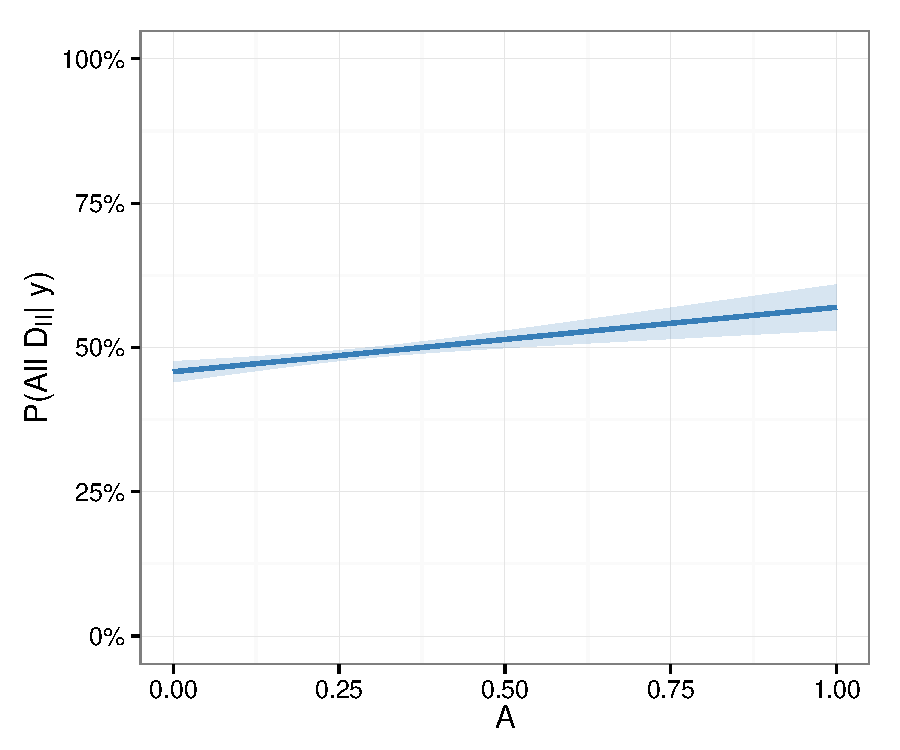
\includegraphics[width=\maxwidth]{figure/ModelResultGph2-1} 

}

\caption[]{$P(\text{All } D_{II})$ as a function of $A$}\label{modModelResultGph2}
\end{figure}


\end{knitrout}

\section{Discussion}
\label{sec:discussion}

\subsection{Implications of the Model}

The findings presented here suggest that our household measure of altruism $A$ appears to be associated with effective discipline strategies. We find no significant effect for a parent's level of efficiency in allocating household resources. However, it remains possible that other parenting decisions may be effected by efficiency. To the extent that effective parenting strategies are correlated with maltreatment, the results of this analysis suggest that relatively simple models of human behavior can explain how families become involved with the child welfare system. Similarly, from a practice perspective, the results of this analysis suggest that some families may be helped more by increases in income or other concrete resources than the sorts of psychotherapeutic interventions which tend to be prevalent in child welfare service plans. For those parents where income is not a concern, this model would suggest that interventions should focus on changing the preferences (i.e. caring and sharing) of parents and households.

What should be clear to the reader at this point is that the model being developed in this paper is implicitly defining child maltreatment as a problem of poverty. While previous researchers have certainly drawn the connection between child welfare and poverty, such literature usually attempts to examine the link between poverty and deviant parental behaviors. Here I take an alternative approach and define neglect based on the manner in which poverty effects a given child (in terms of their well-being) and the biological and social context from which the parental behaviors emanate (resource constraints and level of parental caring). In other words, specific behaviors matter, but only in the context of the causes and consequences of those behaviors.

In defining maltreatment in this manner, I am breaking from established lines of thinking about child neglect. Indeed, many statutes specifically preclude poverty and homelessness as factors to be considered when making legal determinations as to whether or not a given child has been maltreated. While it is understandable that policy makers would not want to hold a parent accountable for factors outside of her control, focusing exclusively on parental behaviors ignores the experience of a child in a given household and the causes of these behaviors. The model presented here also elucidates the dynamic nature of households and the variety of potential intervention points available to the child welfare social work community. 

\subsection{Application of the Model}

The remainder of this paper helps the reader to understand how to apply the results of this analysis to a practice setting by: 1) Increasing the parent's job skills or identifying additional income sources for a household (i.e. mitigating household income constraints $y$), and 2) Changing the parent's choices and preferences whereby more of their existing resources are directed toward their child (i.e. increasing $A$). In order to better understand these intervention points, the following section outlines two hypothetical case examples and describes reasonable service plans stemming from the resource constraint theory of maltreatment.

The first hypothetical family we encounter is a twenty-year old single-mother of a two-year old female. The child has been referred to child protective services by a pediatrician due to an excessive diaper rash which has developed into a fungal infection. The pediatrician believes the proximal cause of the rash to be infrequent changes of the child's soiled diapers. Upon further investigation, the social worker learns that the mother's household is well-below the government's established poverty line. The social worker also learns that the mother clearly understands the guidance from the pediatrician and that the mother is attempting to complete a course of study which will allow her to gain registration as a nurse. The mother had initially secured child care from the grandmother while she was engaged in her coursework. However, the grandmother has recently taken ill and is no longer able to provide care for the child. The mother's teenage sister has been providing some assistance in child care but is not consistently available. 

While a na\"\i ve assessment of the mother's situation may have simply directed her to a parenting education program to teach her to properly diaper the child, a global assessment of the mother's entire situation revealed that the mother understood the directives of the pediatrician but lacked a consistent and qualified child-care provider to tend to the child's needs while the mother was in school. Proceeding from the theory of maltreatment presented here, the social worker's primary goal should be to stabilize the mother's attempts to obtain registration as a nurse as this will provide long-term improvements to the mother's income constraints. The social worker in this example also secured a child care subsidy to provide care for the child in a public child care center and assisted the mother in locating the father of the child in order to start a support maintenance case. The childcare subsidy increases $x_{cm}$ in the child's well-being function and the child support further mitigates the mothers income constraints $y$. 

The second hypothetical household we encounter involves a family of two; another single mother and a 14 year-old female. The family has been referred to the child protection agency due to their dependence on a variety of opiate drugs. The child's material needs appear to be met but she is experiencing excessive truancy and failing marks in her coursework. 

A na\"\i ve assessment of the family's situation may have simply directed the child to a foster placement due to educational neglect. However, in evaluating the situation in the context of the theory of maltreatment articulated here, the social worker assessed that the child, due to her age and apparent ability to self-protect, is actually being provided for above $\bar{w}$. As such, there is no immediate need to disrupt the child's living situation. The household situation described here might be conceptually understood as point $A$ in Figure ~\ref{fig:plot2} above. While the child may not require placement in foster care, the social worker assesses sub-optimal investment in terms of $w_c$ \emph{and} $w_p$. As such, the social worker decides to act preventatively and help the family achieve sobriety for the parent and an optimal education for the child. The social worker thus orders substance abuse services for the parent and a series of multisystemic therapy (MST) sessions for the household which will allow the family to more optimally invest in all of its members within available resources.  

\subsection{Conclusion and Future Directions}

While artificial, these examples provide an illustration as to how the theory of maltreatment presented in this paper can be directly applied to social work practice. While the examples provided are focused on the manner in which individual social workers can use this theoretical model to develop service plans in specific cases, the theory presented here is also applicable to macro-level practice questions. Indeed, the model's explicit focus on resource constraints could serve to inform a child protection system that was less focused on determining whether or not an instance of child maltreatment has taken place and more focused on remedying the resource problems which arguably underlay many reports of child maltreatment. Even when resource constraints are not the problem \emph{per se}, as shown in the second example, the model provides an avenue through which targeted and solution-focused interventions can be identified.  

Despite the usefulness of the model, it does suffer from an implicit assumption of a parent who desires to invest (at least some) resources in their child. The model presented here would suggest that all parents would have a propensity to harm their children under a certain mix of genetics and resource constraints, but that they typically seek to make investments in children which maximize the child's well-being. We know, however, that some parents suffer from various forms of psychopathology which may yield a desire to harm children under any circumstances. Instances of pedophilic sadism seem to be evidence that such individuals do exist. For those individuals, a model of maltreatment focused on the \citet{Kempe1962} ``defect of character'' seems more appropriate than the one presented here. The point of this paper, however, is that we have no reason to believe that such individuals are a normal part of our society or even a normal part of our child welfare system. Such individuals likely represent the margins of both populations and policies and interventions should be developed with this theoretical framework in mind. 

The analysis presented here is generally supportive of a resource constraint theory of child maltreatment. However, we should be clear that the data did not allow us to directly test the model. A direct test of the model would require information on how much parents prefer one form of discipline to another given the relative ``costs'' or ``benefits'' of a given strategy. Thus, one potential future line of research would concern a specific examination of how reduced resource shares translate into decisions about parenting (i.e. a direct attempt to estimate $\alpha_p$. To date, the qualitative choice econometric literature \citep[in the line of][]{Train1986} omits of any examination of how parents choose between discipline strategies. Such projects would more directly test the underlying mechanics of the model presented here. Future research may also seek to explore the line of experiments conducted by \citet{Greene2014}. One could, for example, imagine an brain-imaging experimental in which parent-subjects were placed under cognitive load and asked to make decisions about various parenting strategies. Understanding how parenting decisions are made within the dual-process theory of morality seems critical to our understanding of maltreatment. Finally, additional research is needed (through the direct study of social workers or other means) to understand the societal variability of $\bar{w}$. In other words, since we assume in this model that $\bar{w}$ is societally defined and thus varies across societies, research should be conducted to help us understand precisely how is varies throughout the world; both presently and across time. 

\newpage 
\theendnotes

\newpage
\section*{References}
\bibliographystyle{model5-names}\biboptions{authoryear}
\bibliography{qualpaper}

\end{document}
